\documentclass{article}

\usepackage{graphicx}
\usepackage{tikz}
\usetikzlibrary{calc, spy}
\usepackage[tightpage, active, floats, graphics]{preview}

\begin{document}
\begin{preview}
    \begin{tikzpicture}
        \node (legend) at (0.4, -0.3) {\textsf{Receptive fields}};
        \node (colorbar) at (0.4, -1.3)
        {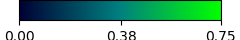
\includegraphics[width=2.4cm]{rf_colorbar.png}};
        \node (legend2) at (0.4, -0.9) {\textsf{\footnotesize Classifier weights}};

        \node (e) at (-.7, -2.3) {\sffamily\bfseries e};
        
        \node (i1780) at (0.4, 1.3)
            {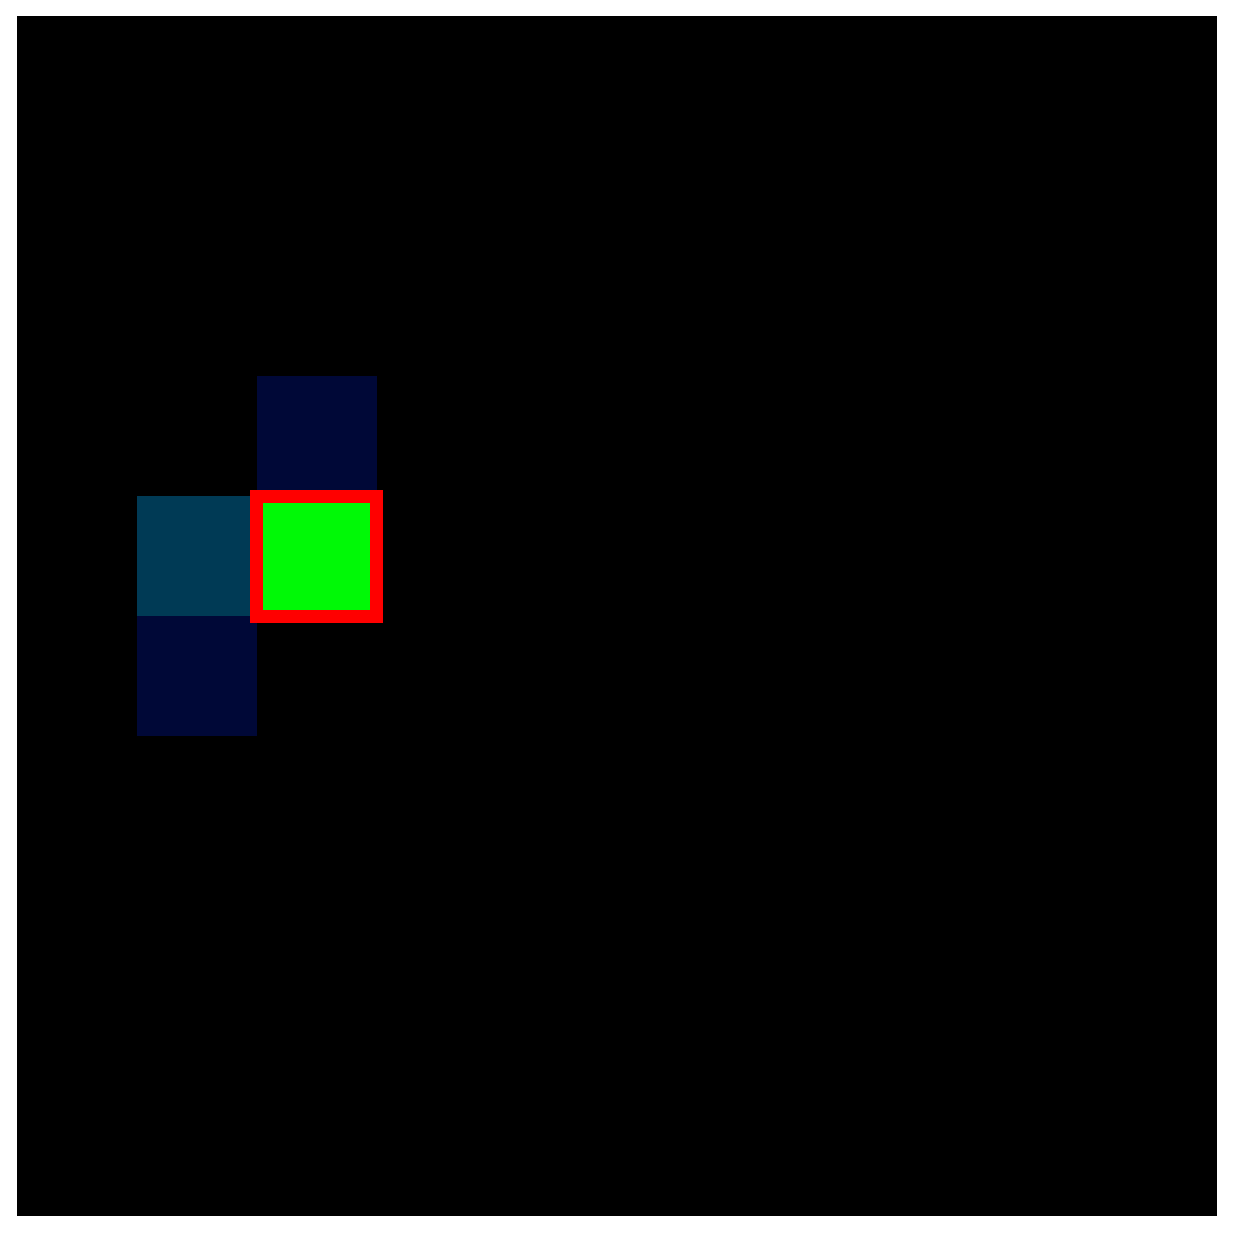
\includegraphics[width=2.4cm]{encoding_1780}};
        \node (i1951) at (3, 1.3)
            {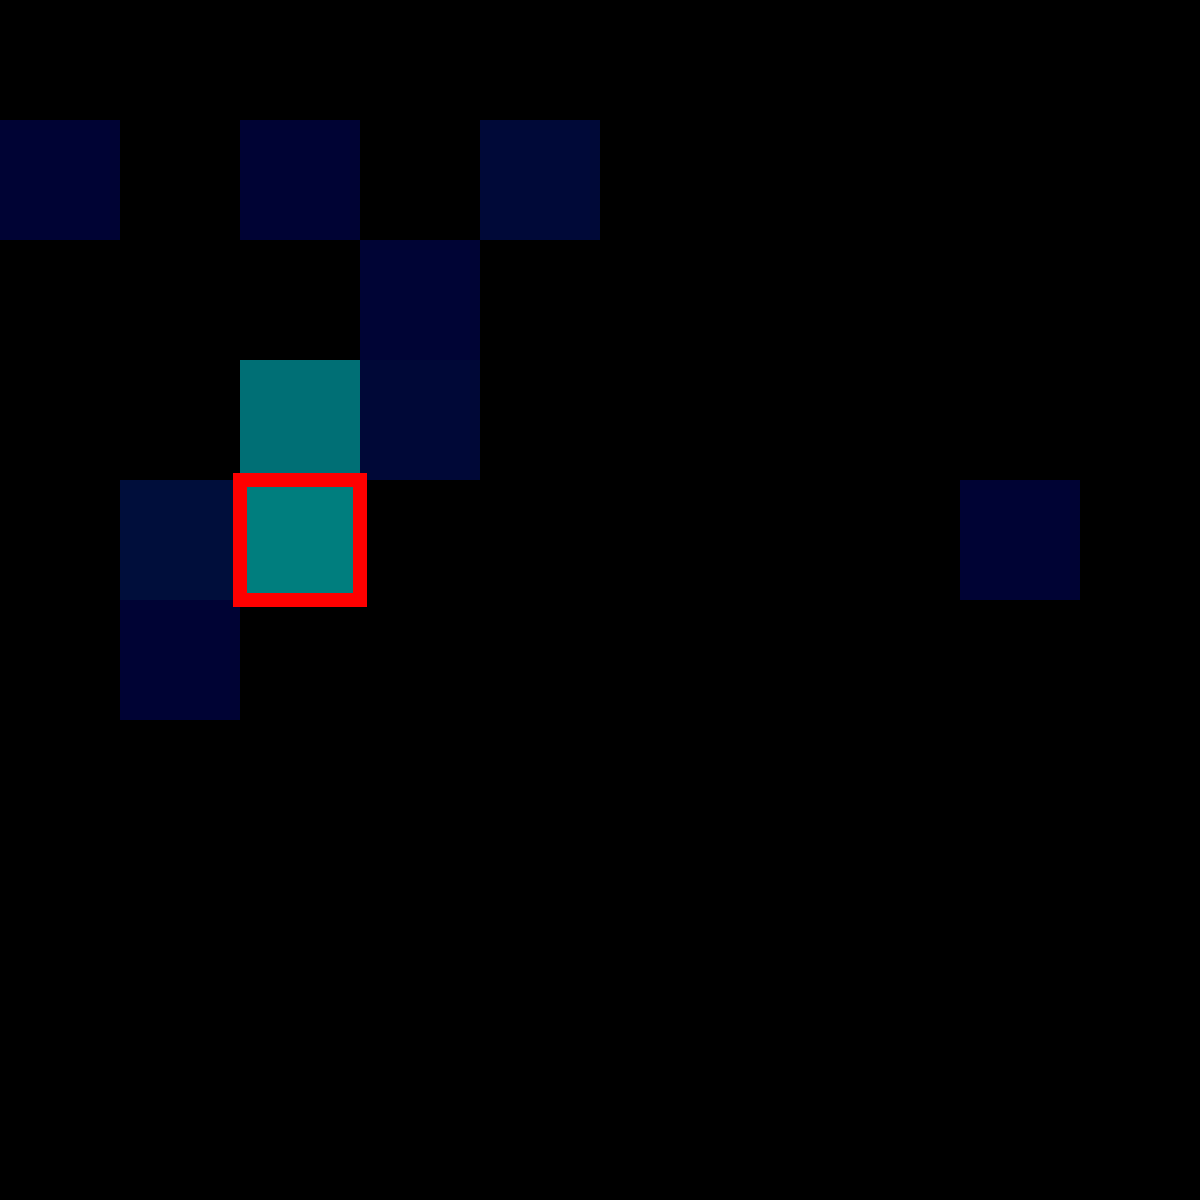
\includegraphics[width=2.4cm]{encoding_1951}};
        \node (i2131) at (5.6, 1.3)
            {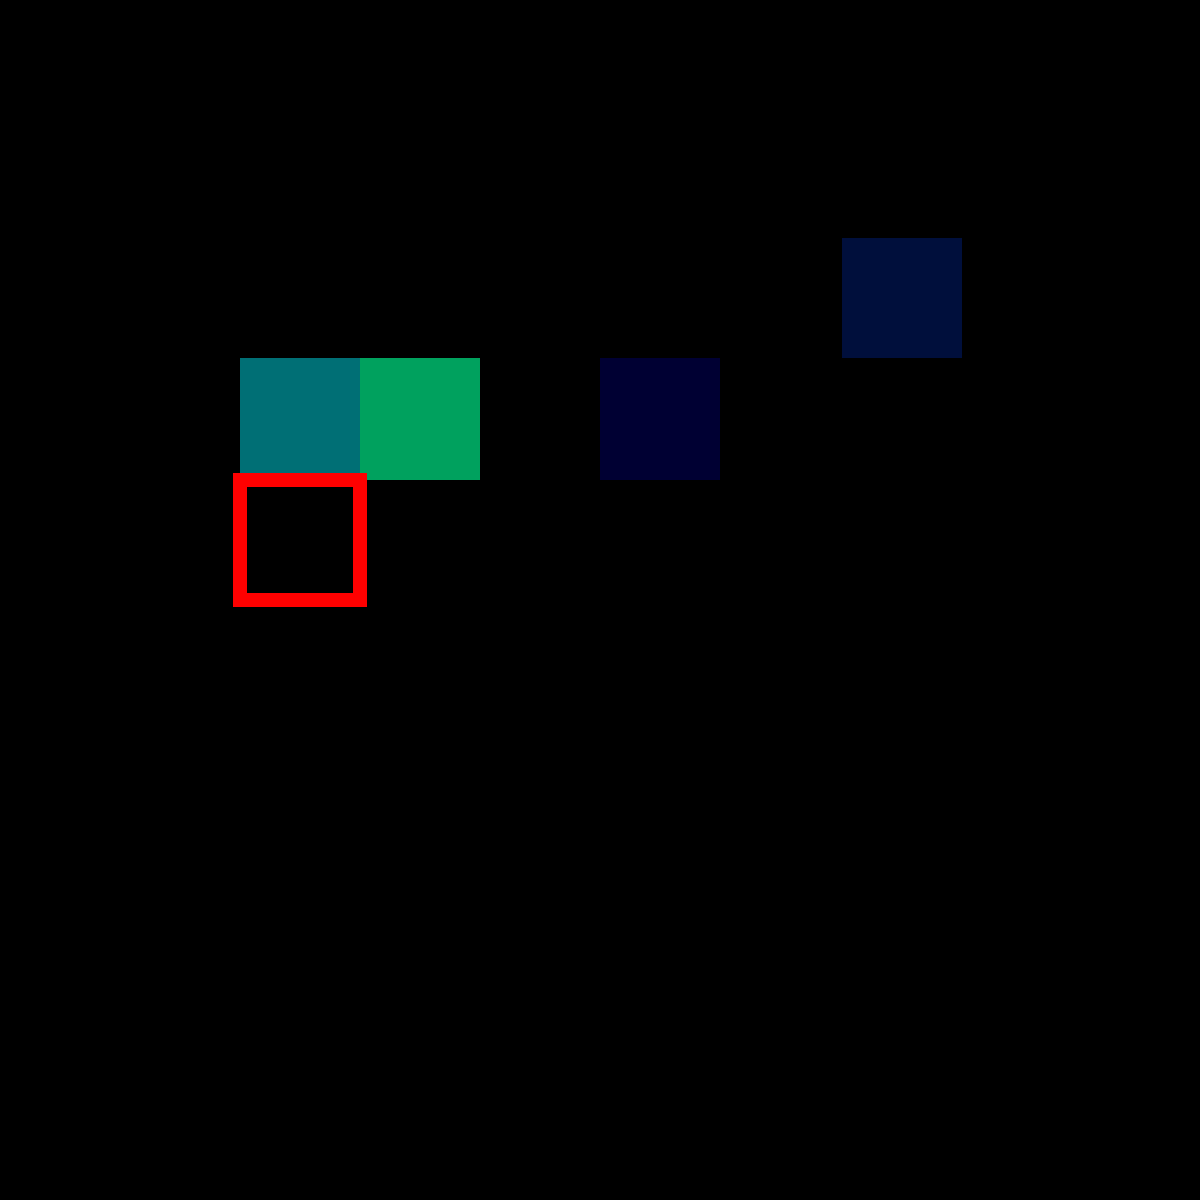
\includegraphics[width=2.4cm]{encoding_2131}};
        \node (i1935) at (3, -1.3)
            {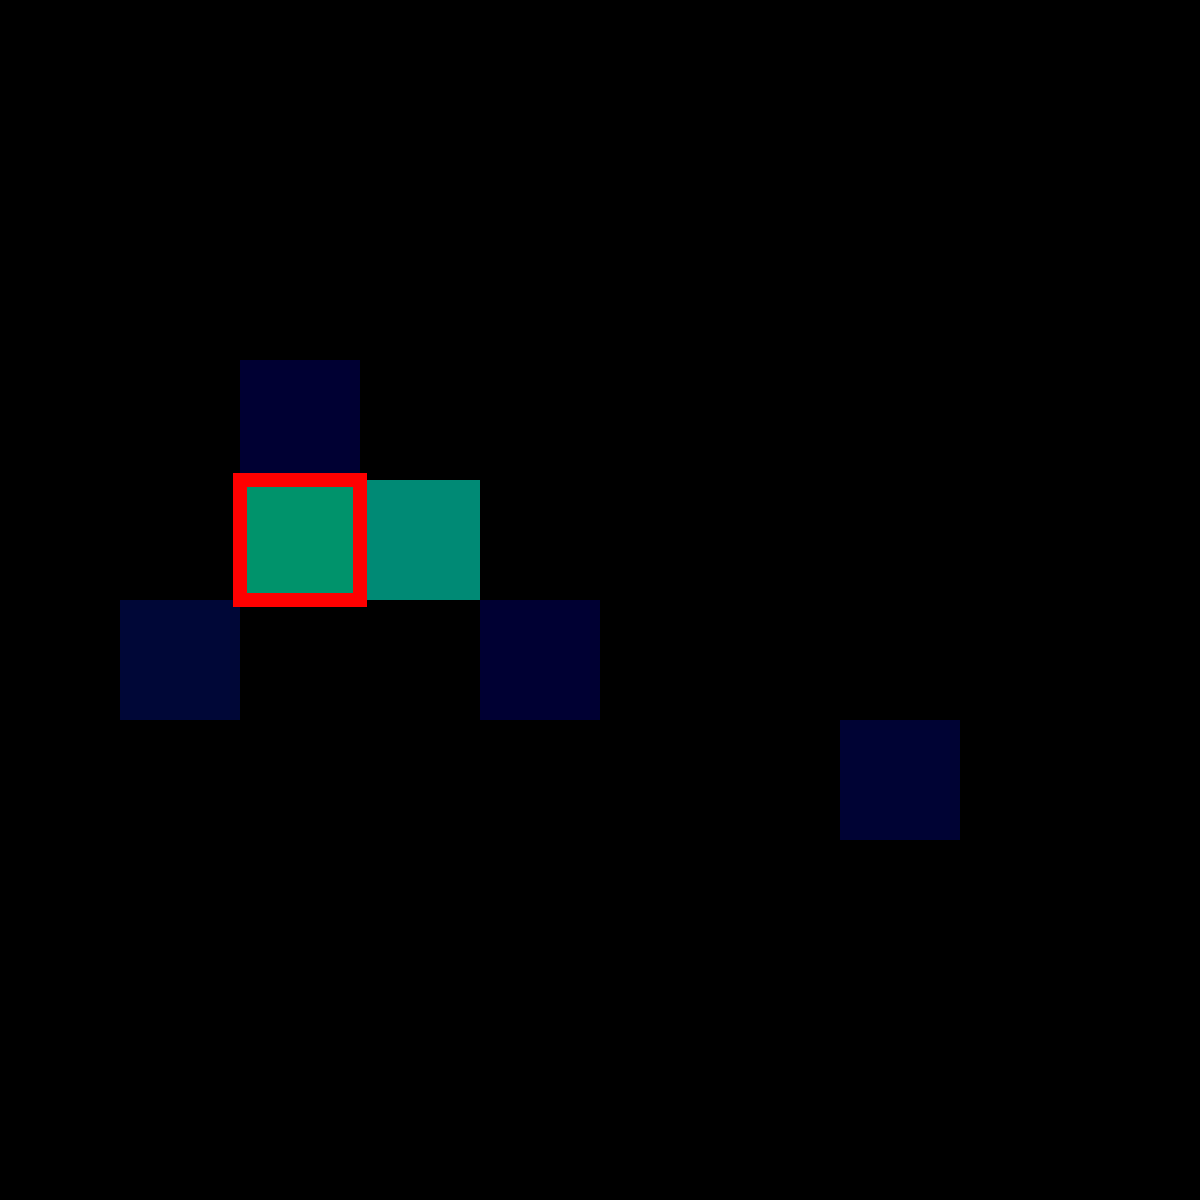
\includegraphics[width=2.4cm]{encoding_1935}};
        \begin{scope}[spy using outlines={blue, circle, line width=3pt,
                magnification=6, size=60, connect spies}]
                \node at(9.5, 0)
                {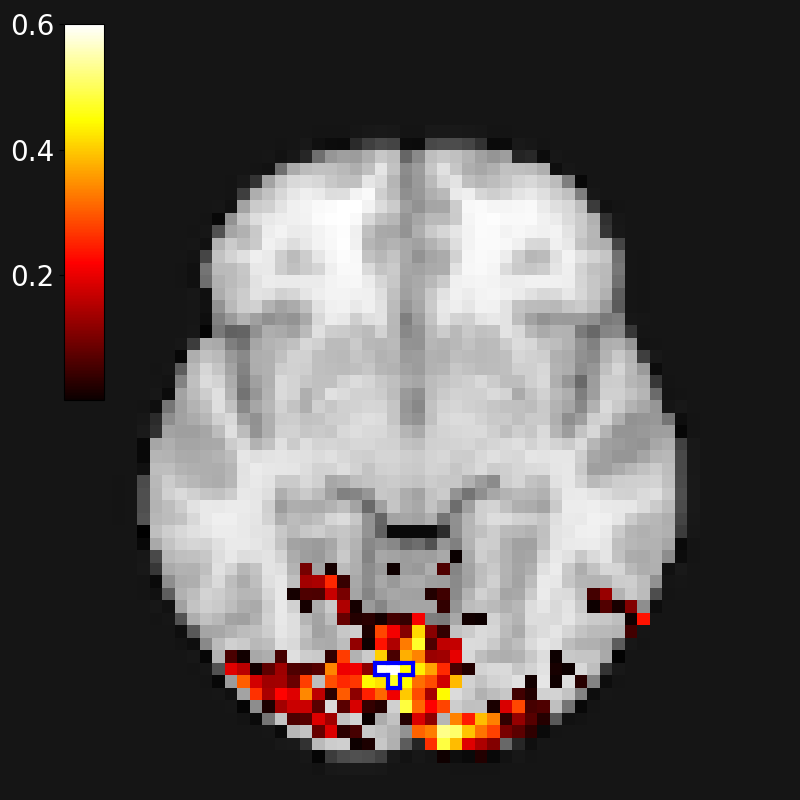
\includegraphics[width=5cm]{encoding_scores.png}};
            \spy [width=3cm, height=3cm, line width=3pt, spy connection path={\draw[line
            width=2pt, blue] (tikzspyonnode) -- (tikzspyinnode);}]
            on (9.46, -1.7) in node (a) [line width=4pt] (a) at (10.7,1) (a) {};
        \end{scope} 
        \node (f) at (7.2, -2.3) {\color{white}\sffamily\bfseries f};

    \end{tikzpicture}
\end{preview}
\end{document}
